\documentclass[border=4pt]{standalone}
\usepackage{tikz}
\usetikzlibrary{arrows.meta,positioning,shapes.geometric}
\begin{document}
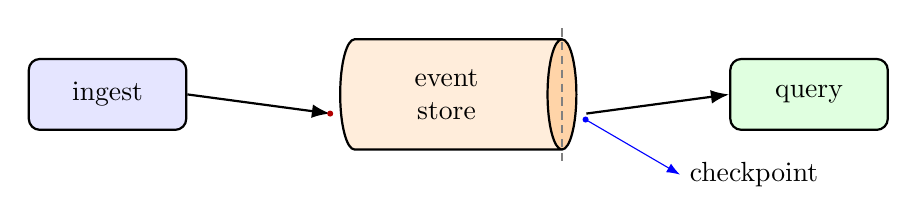
\begin{tikzpicture}[
  >=Latex,
  node distance=18mm,
  stage/.style={draw,thick,rounded corners,minimum width=20mm,minimum height=9mm},
  store/.style={cylinder,shape aspect=.42,draw,thick,minimum width=14mm,
    minimum height=30mm,outer sep=4pt,cylinder uses custom fill,
    cylinder body fill=orange!14,cylinder end fill=orange!34,align=center}
]
  \node[stage,fill=blue!10] (ingest) {ingest};
  \node[store,right=of ingest] (store) {event\\store};
  \node[stage,fill=green!12,right=of store] (query) {query};

  \draw[-Latex,thick] (ingest.east) -- (store.mid west);
  \draw[-Latex,thick] (store.mid east) -- (query.west);
  \draw[-Latex,blue] (store.base east) -- ++(12mm,-7mm)
    node[right,black] {checkpoint};
  \draw[densely dashed,gray] (store.before top) -- (store.after top);
  \fill[blue] (store.base east) circle (1.1pt);
  \fill[red!70!black] (store.mid west) circle (1.1pt);
\end{tikzpicture}
\end{document}
